\section{Gasphasenabscheidungen}
\label{depositions}

\todo[inline]{Anmerkung von Jörg: Mehr Referenzen zu den Prozessen, spätestens bei ALD}

Gasphasenabscheidungen sind Herstellungsverfahren für dünne Schichten, bei denen durch physikalische oder chemische Prozesse aus einer Gasphase eine dünne Schicht auf einer Oberfläche aufgewachsen wird.
Bei den hier untersuchten Arten von Gasphasenabscheidungen handelt es sich um \textbf{Physikalische Gasphasenabscheidung} (PVD, Physical Vapor Deposition), \textbf{Chemische Gasphasenabscheidung} (CVD, Chemical Vapor Deposition) und \textbf{Atomlagenabscheidung} (ALD, Atomic Layer Deposition), die im folgenden vorgestellt werden.

Allen Verfahren ist gemein, dass einzelne Atome oder Moleküle aus der Gasphase auf der Oberfläche auftreffen, dort physikalisch oder chemisch adsorbiert werden und so mit vorhersehbarer Rate eine dünne Schicht eines gewünschten Materiales bilden.
\todo{Satz klingt komisch}Dennoch hat jeder Prozess seine eigenen Eigenschaften, die es ihm ermöglichen, verschiedene Materialarten mit unterschiedlicher Kontrolle über die Qualität aufzuwachsen.
Tabellen~\ref{tab:deposition-comparison} und~\ref{tab:deposition-materials} sollen einen kurzen Überblick darüber verschaffen, bevor die Prozesse im einzelnen vorgestellt werden.
Alle Prozesse finden in speziellen Abscheidungskammern oder Reaktoren statt, über die Abbildung~\ref{fig:reactors} einen kurzen Überblick geben soll.

\begin{figure}
  \captionsetup[subfigure]{format=plain}
  \def\chamberwidth{0.3\textwidth}
  \def\subcaptionwidth{0.65\textwidth}

  \parbox[c]{\chamberwidth}{
    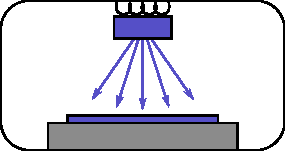
\includegraphics[width=\linewidth]{reactors-z}
  }\hfill
  \parbox[c]{\subcaptionwidth}{
    \subcaption{Evaporations-Kammer (PVD):
      Material wird thermisch oder elektrisch in einer Vakuumkammer verdampft und kondensiert auf dem gegenüber liegenden Substrat als dünne Schicht.
    }
  }

  \vspace{1em}

  \parbox[c]{\chamberwidth}{
    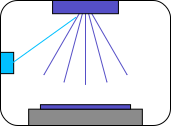
\includegraphics[width=\linewidth]{reactors-a}
  }\hfill
  \parbox[c]{\subcaptionwidth}{
    \subcaption{Sputter-Kammer (PVD):
      Ein Elektronen- oder Ionenstrahl (links) schlägt Atome aus dem Target (oben), die sich auf dem Substrat (unten) als dünne Schicht absetzen.
    }
  }

  \vspace{1em}

  \parbox[c]{\chamberwidth}{
    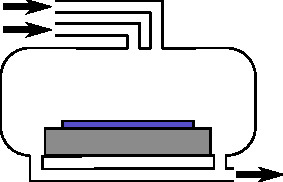
\includegraphics[width=\linewidth]{reactors-b}
  }\hfill
  \parbox[c]{\subcaptionwidth}{
    \subcaption{Injektions-Kammer (CVD, ALD):
      Precursorgase strömen über ein Substrat, auf dem sie durch chemische Reaktionen dünne Schichten abscheiden.
      Nebenprodukte der Oberflächenreaktionen werden mit dem Gasstrom aus dem Reaktor gespült.
    }
  }

  \vspace{1em}

  \parbox[c]{\chamberwidth}{
    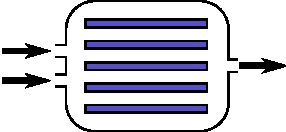
\includegraphics[width=\linewidth]{reactors-c}
  }\hfill
  \parbox[c]{\subcaptionwidth}{
    \subcaption{Batch-Reaktor (CVD, ALD):
      Wie Injektions-Kammer, aber mit Stapeln von Substraten.
      Effiziente Methode zur industriellen Beschichtung per CVD oder ALD.
    }
  }

  \caption[Arten von Abscheidungskammern]{
    Arten von Abscheidungskammern für PVD, CVD und ALD\cite{granneman_batch_2007}.
  }
  \label{fig:reactors}
\end{figure}

\begin{table}
  \oddrowcolors
  \caption[Eigenschaften von PVD-, CVD- und ALD-Prozessen]{Eigenschaften von PVD-, CVD- und ALD-Prozessen}
  \label{tab:deposition-comparison}
  \begin{tabularx}{\textwidth}{|Xccc|}
    \hline
    \textbf{Eigenschaften} & \textbf{PVD}    & \textbf{CVD}       & \textbf{ALD}         \\
    \hline
    reaktiv                &                 & \cmark             & \cmark               \\
    kontinuierlich         & \cmark          & \cmark             & zyklisch             \\
    Gas-Edukte             & Atome, Moleküle & Precursor-Moleküle & Precursor-Moleküle   \\
    \# Edukte              & 1               & 1+                 & 2+                   \\
    Nebenprodukte          &                 & \cmark             & \cmark               \\
    Wachstumsrate          & $\sim t$        & $\sim t$           & $\sim n_\text{cyc.}$ \\
    \hline
  \end{tabularx}
\end{table}

\begin{table}
  \begin{threeparttable}
    \caption[Auswahl möglicher Produkte von PVD, CVD und ALD]{
      Auswahl möglicher Produkte von PVD, CVD und ALD.
      Weitere Produkte und Precursor finden sich in den Referenzen für PVD\cite{mattox_handbook_2010,helmersson_ionized_2006}, CVD\cite{pierson_handbook_1999} und ALD\cite{puurunen_surface_2005,elliott_atomic-scale_2012}.
    }
    \label{tab:deposition-materials}
    \begin{tabularx}{\textwidth}{XcX}
     & \begin{minipage}[t]{0.55\textwidth}
         \oddrowcolors
         \centering
         \begin{tabular}{|lccc|}
           \hline
           \textbf{Produkt} & \textbf{PVD} & \textbf{CVD} & \textbf{ALD}      \\
           \hline
           Metalle          & \cmark       & \cmark       & (\cmark)\tnote{a} \\
           Legierungen      & \cmark       & \cmark       & ~                 \\
           Metalloxide      & ~            & \cmark       & \cmark            \\
           Nitride          & ~            & \cmark       & \cmark            \\
           Chloride         & ~            & \cmark       & \cmark            \\
           Silizium         & \cmark       & \cmark       & \cmark            \\
           Siliziumoxid     & ~            & \cmark       & \cmark            \\
           Diamant          & ~            & \cmark       & \cmark            \\
           \hline
         \end{tabular}
       \end{minipage}
    & \\
    \end{tabularx}
    \begin{tablenotes}
    \item[a] Metall-ALD ist zwar möglich, aber mit vielen Hürden verbunden.\todo[inline]{sinnvoller Satz!}
    \end{tablenotes}
  \end{threeparttable}
\end{table}

\subsection{Physikalische Gasphasenabscheidung}

Physikalische Gasphasenabscheidungen (PVD, Physical Vapor Deposition) sind eine grundlegende Art von Abscheidungsprozessen, bei denen einzelne Atome nichtreaktiv auf einer Oberfläche adsorbieren.
Zu ihnen zählt neben der thermischen oder elektrischen Evaporation auch Sputtering, bei dem aus einem Block des gewünschten Materiales (Target) per Elektronen- oder Ionenstrahl kontinuierlich Atome herausgeschlagen werden, die sich dann auf dem Substrat absetzen und dort zu einer dünnen Schicht verbinden.
Anhand der Energien der herausschlagenden Partikel, dem Teilchenstrom und der Substrattemperatur lässt sich dabei die Wachstumsrate und Qualität des abgeschiedenen Dünnfilmes beeinflussen.
Durch die geradlinige Ausbreitung der aus dem Target evaporierten oder geschlagenen Partikel lassen sich zwar dünne, konforme Schichten auf glatten Substraten erzeugen\cite{svorcik_annealing_2011}, doch wird dadurch eine ebenmäßige Beschichtung komplizierter Geometrien verhindert.
Die Abscheidung gemischter Systeme wie Legierungen und mehrlagigen Schichten wird hierbei durch Nutzung mehrerer Targets ermöglicht\cite{cammarata_nanoindentation_1990}.

\subsection{Chemische Gasphasenabscheidung}

Während einer Chemischen Gasphasenabscheidung (CVD, Chemical Vapor Deposition) adsorbieren sogenannte Precursormoleküle physikalisch auf dem Substrat und reagieren im Anschluss mit an der Oberfläche befindlichen Atomen.
Dabei werden entweder Teile des Precursors auf der Oberfläche hinterlassen oder von vorherigen Reaktionen verbliebene Precursorliganden von der Oberfläche entfernt, wodurch bei entsprechender Prozessgestaltung gewünschte Stöchiometrien und Bindungen bevorzugt gebildet werden.
Abbildung~\ref{fig:ald-schema} stellt diese Vorgehensweise für ALD-Prozesse dar, die eine Spezialisierung von CVD-Prozessen sind und im nächsten Abschnitt vorgestellt werden.
Da es sich um einen kontinuierlichen Prozess handelt, befinden sich meist zwei Precursorgase gleichzeitig im Reaktor, wo sie idealerweise erst auf der Oberfläche miteinander reagieren, da Reaktionen zwischen ihnen in der Gasphase neben einem erhöhtem Gasverbrauch zu Verunreinigungen und Partikelbildung führen können.

Für erfolgreiche Abscheidungsprozesse ist es wichtig, neben passenden Umgebungsbedingungen auch Precursormoleküle zu wählen, die einerseits eine hohe Qualität des Filmes gewährleisten, andererseits kompakt genug sind, um hohe Wachstumsraten zu ermöglichen.
Zudem sollten die gasförmigen Nebenprodukte inert sein, um nicht mit der Oberfläche oder der Reaktorwand zu reagieren, während sie mit dem kontinuierlichen Gasfluss aus dem Reaktor gespült werden.
Auch eine physikalische Adsorption der Nebenprodukte auf der Oberfläche kann den Dünnfilm verunreinigen.
Dabei sind stets die Prozesstemperaturen, -drücke, Reaktionsbarrieren und die Stabilität aller involvierten Moleküle zu beachten, wodurch auch \todo{Anmerkung von Jörg: das gilt an sich für alle Abscheideprozesse}alle chemischen Gasphasenabscheidungsprozesse oft in monatelanger Arbeit optimiert werden müssen.
Wie bei PVD lässt sich die Schichtdicke auf mehrere Nanometer genau kontrollieren, was hinsichtlich einer gegenüber ALD vergleichsweise hohen \todo{ref}Wachstumsrate für viele Anwendungen ausreichend ist.

\todo[inline]{Abbildung Beispiel Precursor-Moleküle}
\missingfigure{Beispiel Precursor-Moleküle}

\subsection{Atomlagenabscheidung}

\begin{figure}
  \centering
  \def\svgwidth{\textwidth}
  \input{img/ald-schema.pdf_tex}
  \caption[Schema eines vollständigen ALD-Zyklus']{
    Schema eines vollständigen ALD-Zyklus':
    Pulse von reaktiven Precursorgasen A (a) und B (c) zwischen Spül-Schritten mit inertem Gas (b) und (d).
  }
  \label{fig:ald-schema}
\end{figure}

Als Variation einer Chemischen Gasphasenabscheidung entstanden Atomlagenabscheidungen (ALD, Atomic Layer Deposition) mit dem Ziel\todo{Referenz auf 50 Jahre altes Paper?}, konforme dünne Schichten kontrolliert in einzelnen Atomlagen mit Sub-Nanometer-Genauigkeit der Schichtdicke aufwachsen zu lassen.
Dazu werden zwei Precursorgase wechselweise in separaten Schritten (Halbzyklen) in den Reaktor geleitet, wo sie wie bei CVD-Prozessen mit der Oberfläche reagieren und so langsam eine Schicht bilden (Abbildung~\ref{fig:ald-schema}).
Zwischen den Precursorschritten entfernen Spülschritte mit inertem Gas verbleibende Precursormoleküle und Nebenprodukte aus dem Reaktor und verhindern so gleichzeitige Reaktionen beider Precursorgase.
So werden einerseits Gasphasenreaktionen vermieden, andererseits limitiert die Sättigung der Oberfläche mit Precursorliganden in jedem Precursorschritt die Zunahme der Dicke pro Zyklus.
Die Wachstumsrate aus den kontinuierlichen Prozessen wird daher von dem Growth-per-Cycle-Wert (GPC) abgelöst, der angibt, wie viel eine Schicht im Schnitt pro Zyklus wächst.
Über die Zahl der Zyklen lässt sich somit die Dicke der gewachsenen Schicht genauer als mit kontinuierlichen Abscheidungen steuern, was sich aber in langsameren Abscheidungsprozessen äußert.

Anders als der Name des Prozesses vermuten lässt, werden aufgrund sterischer Hinderung (Abbildung~\ref{fig:sterichindrance}) der Precursorliganden keine kompletten Atomlagen in jedem Zyklus aufgebracht.
Üblicherweise erreichen ALD-Prozesse maximal \SI{35}{\percent} einer Monolage pro Zyklus\cite{ylilammi_monolayer_1996}, doch sinkt dieser Wert mit der Größe der Precursormoleküle aufgrund der erweiterten sterischen Hinderung.
Die Suche nach möglichen Precursorpaaren und Prozessparametern unterliegt ansonsten gleichen Anforderungen wie bei CVD.
Eine ausführlichere Übersicht zu Atomlagenabscheidungen und zu möglichen Precursorpaaren für verschiedene Materialien findet sich in Referenz~\cite{puurunen_surface_2005}.

\begin{figure}
  \centering
  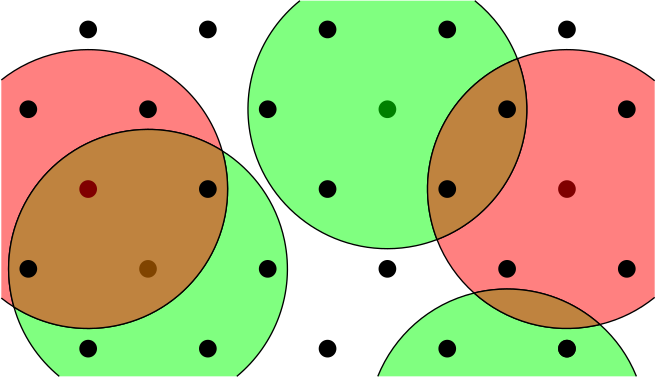
\includegraphics[width=0.5\textwidth]{sterichindrance_noalpha}
  \caption[Sterische Hinderung auf einem Gitter]{
    Sterische Hinderung auf einem Gitter:
    Adsorbierte Liganden schirmen benachbarte Gitterpunkte von weiteren Precursormolekülen ab.
  }
  \label{fig:sterichindrance}
\end{figure}

\subsection{Simulation von Gasphasenabscheidungen}

\begin{table}
  \oddrowcolors
  \caption{Überblick über Methoden zur Simulation von Gasphasenabscheidungen}
  \label{tab:deposition-simulations}
  \begin{tabularx}{\textwidth}{|XXlX|}
    \hline
    \textbf{Methode}                   & \textbf{Anwendungsfeld}                   & \textbf{Größenordnung} & \textbf{Grundlagen}                 \\
    \hline
    Computational Fluid Dynamics (CFD) & Gasfluss in Reaktoren                     & makroskopisch          & Navier-Stokes-Gl., Reaktionskinetik \\
    Kinetic Monte Carlo (KMC)          & Reaktionskinetik                          & mikroskopisch          & Reaktionsraten, Simulationsgitter   \\
    Molekular\-dynamik (MD)            & thermische und strukturelle Eigenschaften & \num{<1000000} Atome   & klassische Interaktionspotentiale   \\
    Dichte\-funktional\-theorie (DFT)  & atomistische Struktur, Reaktionspfade     & \num{<1000} Atome      & Elektronendichten                   \\
    \hline
  \end{tabularx}
  \todo[inline]{Eventuell einen Hinweis auf FEM hinzufügen}
\end{table}

\todo[inline]{fig:methodscales}
\missingfigure{fig:methodscales}

Für die Simulation von Gasphasenabscheidungen stehen verschiedene numerische Methoden zur Verfügung, welche die Darstellung auf unterschiedlichen Zeit- und Größenordnungen ermöglichen (Tabelle~\ref{tab:deposition-simulations})\todo{fig:methodscales}.
Jede dieser Methoden basiert auf anderen Annahmen und Formulierungen, so dass sich ihre Anwendungsgebiete zwar nur marginal überschneiden, aber der Transfer von Ergebnissen zwischen den Methoden zu präziseren Vorhersagen führen kann.
So können FEM-Reaktorsimulationen den Gasverbrauch an charakteristischen Punkten der Oberfläche durch KMC-Simulationen ermitteln, welche wiederum auf DFT-Daten für Reaktionsraten und -energien zurück greift.
Bisherige Simulationen verzichten meist auf ein strukturelle Betrachtungen der abgeschiedenen Schicht, wie sie etwa mit molekulardynamischen Rechnungen möglich werden.
Gerade für Anwendungen in der Nanoelektronik sind die strukturellen Eigenschaften der Schichten aber eng mit der benötigten Funktion (bechanische und elektronische Eigenschaften) verknüpft, so dass eine Vorhersage der strukturellen Eigenschaften mittel Simulation wünschenswert ist.
